\documentclass[12pt,a4paper]{article}

\usepackage[a4paper,text={16.5cm,25.2cm},centering]{geometry}
\usepackage{lmodern}
\usepackage{amssymb,amsmath}
\usepackage{bm}
\usepackage{graphicx}
\usepackage{microtype}
\usepackage{hyperref}
\usepackage{mhchem}
\setlength{\parindent}{0pt}
\setlength{\parskip}{1.2ex}
\setcounter{secnumdepth}{0}% % Turns off numbering for sections
\hypersetup
       {
           colorlinks=TRUE,
           linkcolor=black,
           citecolor=blue,
           urlcolor=blue
       }

\usepackage{upquote}
\usepackage{listings}
\usepackage{xcolor}
\lstset{
    basicstyle=\ttfamily\footnotesize,
    upquote=true,
    breaklines=true,
    breakindent=0pt,
    keepspaces=true,
    showspaces=false,
    columns=fullflexible,
    showtabs=false,
    showstringspaces=false,
    escapeinside={(*@}{@*)},
    extendedchars=true,
}
\newcommand{\HLJLt}[1]{#1}
\newcommand{\HLJLw}[1]{#1}
\newcommand{\HLJLe}[1]{#1}
\newcommand{\HLJLeB}[1]{#1}
\newcommand{\HLJLo}[1]{#1}
\newcommand{\HLJLk}[1]{\textcolor[RGB]{148,91,176}{\textbf{#1}}}
\newcommand{\HLJLkc}[1]{\textcolor[RGB]{59,151,46}{\textit{#1}}}
\newcommand{\HLJLkd}[1]{\textcolor[RGB]{214,102,97}{\textit{#1}}}
\newcommand{\HLJLkn}[1]{\textcolor[RGB]{148,91,176}{\textbf{#1}}}
\newcommand{\HLJLkp}[1]{\textcolor[RGB]{148,91,176}{\textbf{#1}}}
\newcommand{\HLJLkr}[1]{\textcolor[RGB]{148,91,176}{\textbf{#1}}}
\newcommand{\HLJLkt}[1]{\textcolor[RGB]{148,91,176}{\textbf{#1}}}
\newcommand{\HLJLn}[1]{#1}
\newcommand{\HLJLna}[1]{#1}
\newcommand{\HLJLnb}[1]{#1}
\newcommand{\HLJLnbp}[1]{#1}
\newcommand{\HLJLnc}[1]{#1}
\newcommand{\HLJLncB}[1]{#1}
\newcommand{\HLJLnd}[1]{\textcolor[RGB]{214,102,97}{#1}}
\newcommand{\HLJLne}[1]{#1}
\newcommand{\HLJLneB}[1]{#1}
\newcommand{\HLJLnf}[1]{\textcolor[RGB]{66,102,213}{#1}}
\newcommand{\HLJLnfm}[1]{\textcolor[RGB]{66,102,213}{#1}}
\newcommand{\HLJLnp}[1]{#1}
\newcommand{\HLJLnl}[1]{#1}
\newcommand{\HLJLnn}[1]{#1}
\newcommand{\HLJLno}[1]{#1}
\newcommand{\HLJLnt}[1]{#1}
\newcommand{\HLJLnv}[1]{#1}
\newcommand{\HLJLnvc}[1]{#1}
\newcommand{\HLJLnvg}[1]{#1}
\newcommand{\HLJLnvi}[1]{#1}
\newcommand{\HLJLnvm}[1]{#1}
\newcommand{\HLJLl}[1]{#1}
\newcommand{\HLJLld}[1]{\textcolor[RGB]{148,91,176}{\textit{#1}}}
\newcommand{\HLJLs}[1]{\textcolor[RGB]{201,61,57}{#1}}
\newcommand{\HLJLsa}[1]{\textcolor[RGB]{201,61,57}{#1}}
\newcommand{\HLJLsb}[1]{\textcolor[RGB]{201,61,57}{#1}}
\newcommand{\HLJLsc}[1]{\textcolor[RGB]{201,61,57}{#1}}
\newcommand{\HLJLsd}[1]{\textcolor[RGB]{201,61,57}{#1}}
\newcommand{\HLJLsdB}[1]{\textcolor[RGB]{201,61,57}{#1}}
\newcommand{\HLJLsdC}[1]{\textcolor[RGB]{201,61,57}{#1}}
\newcommand{\HLJLse}[1]{\textcolor[RGB]{59,151,46}{#1}}
\newcommand{\HLJLsh}[1]{\textcolor[RGB]{201,61,57}{#1}}
\newcommand{\HLJLsi}[1]{#1}
\newcommand{\HLJLso}[1]{\textcolor[RGB]{201,61,57}{#1}}
\newcommand{\HLJLsr}[1]{\textcolor[RGB]{201,61,57}{#1}}
\newcommand{\HLJLss}[1]{\textcolor[RGB]{201,61,57}{#1}}
\newcommand{\HLJLssB}[1]{\textcolor[RGB]{201,61,57}{#1}}
\newcommand{\HLJLnB}[1]{\textcolor[RGB]{59,151,46}{#1}}
\newcommand{\HLJLnbB}[1]{\textcolor[RGB]{59,151,46}{#1}}
\newcommand{\HLJLnfB}[1]{\textcolor[RGB]{59,151,46}{#1}}
\newcommand{\HLJLnh}[1]{\textcolor[RGB]{59,151,46}{#1}}
\newcommand{\HLJLni}[1]{\textcolor[RGB]{59,151,46}{#1}}
\newcommand{\HLJLnil}[1]{\textcolor[RGB]{59,151,46}{#1}}
\newcommand{\HLJLnoB}[1]{\textcolor[RGB]{59,151,46}{#1}}
\newcommand{\HLJLoB}[1]{\textcolor[RGB]{102,102,102}{\textbf{#1}}}
\newcommand{\HLJLow}[1]{\textcolor[RGB]{102,102,102}{\textbf{#1}}}
\newcommand{\HLJLp}[1]{#1}
\newcommand{\HLJLc}[1]{\textcolor[RGB]{153,153,119}{\textit{#1}}}
\newcommand{\HLJLch}[1]{\textcolor[RGB]{153,153,119}{\textit{#1}}}
\newcommand{\HLJLcm}[1]{\textcolor[RGB]{153,153,119}{\textit{#1}}}
\newcommand{\HLJLcp}[1]{\textcolor[RGB]{153,153,119}{\textit{#1}}}
\newcommand{\HLJLcpB}[1]{\textcolor[RGB]{153,153,119}{\textit{#1}}}
\newcommand{\HLJLcs}[1]{\textcolor[RGB]{153,153,119}{\textit{#1}}}
\newcommand{\HLJLcsB}[1]{\textcolor[RGB]{153,153,119}{\textit{#1}}}
\newcommand{\HLJLg}[1]{#1}
\newcommand{\HLJLgd}[1]{#1}
\newcommand{\HLJLge}[1]{#1}
\newcommand{\HLJLgeB}[1]{#1}
\newcommand{\HLJLgh}[1]{#1}
\newcommand{\HLJLgi}[1]{#1}
\newcommand{\HLJLgo}[1]{#1}
\newcommand{\HLJLgp}[1]{#1}
\newcommand{\HLJLgs}[1]{#1}
\newcommand{\HLJLgsB}[1]{#1}
\newcommand{\HLJLgt}[1]{#1}


\begin{document}

\section{Jump process using Gillespie.jl}
Simon Frost (@sdwfrost), 2020-04-27

\subsection{Introduction}
This implementation of a jump process uses \href{https://github.com/sdwfrost/Gillespie.jl}{\texttt{Gillespie.jl}} rather than \texttt{DifferentialEquations.jl}, which gives (slightly) better performance.

\subsection{Libraries}
We will need to install the (unregistered) package, \texttt{Gillespie.jl}


\begin{lstlisting}
[?25l[?25h
\end{lstlisting}


The library can now be loaded along with the other packages.



\subsection{Transitions}
\texttt{Gillespie.jl} expects a single function that returns a vector of all the rates.


\begin{lstlisting}
(*@\HLJLk{function}@*) (*@\HLJLnf{sir{\_}rates}@*)(*@\HLJLp{(}@*)(*@\HLJLn{x}@*)(*@\HLJLp{,}@*)(*@\HLJLn{parms}@*)(*@\HLJLp{)}@*)
  (*@\HLJLp{(}@*)(*@\HLJLn{S}@*)(*@\HLJLp{,}@*)(*@\HLJLn{I}@*)(*@\HLJLp{,}@*)(*@\HLJLn{R}@*)(*@\HLJLp{)}@*) (*@\HLJLoB{=}@*) (*@\HLJLn{x}@*)
  (*@\HLJLp{(}@*)(*@\HLJLn{\ensuremath{\beta}}@*)(*@\HLJLp{,}@*)(*@\HLJLn{c}@*)(*@\HLJLp{,}@*)(*@\HLJLn{\ensuremath{\gamma}}@*)(*@\HLJLp{)}@*) (*@\HLJLoB{=}@*) (*@\HLJLn{parms}@*)
  (*@\HLJLn{N}@*) (*@\HLJLoB{=}@*) (*@\HLJLn{S}@*)(*@\HLJLoB{+}@*)(*@\HLJLn{I}@*)(*@\HLJLoB{+}@*)(*@\HLJLn{R}@*)
  (*@\HLJLn{infection}@*) (*@\HLJLoB{=}@*) (*@\HLJLn{\ensuremath{\beta}}@*)(*@\HLJLoB{*}@*)(*@\HLJLn{c}@*)(*@\HLJLoB{*}@*)(*@\HLJLn{I}@*)(*@\HLJLoB{/}@*)(*@\HLJLn{N}@*)(*@\HLJLoB{*}@*)(*@\HLJLn{S}@*)
  (*@\HLJLn{recovery}@*) (*@\HLJLoB{=}@*) (*@\HLJLn{\ensuremath{\gamma}}@*)(*@\HLJLoB{*}@*)(*@\HLJLn{I}@*)
  (*@\HLJLp{[}@*)(*@\HLJLn{infection}@*)(*@\HLJLp{,}@*)(*@\HLJLn{recovery}@*)(*@\HLJLp{]}@*)
(*@\HLJLk{end}@*)(*@\HLJLp{;}@*)
\end{lstlisting}


The transitions are defined as an array of arrays.


\begin{lstlisting}
(*@\HLJLn{sir{\_}transitions}@*) (*@\HLJLoB{=}@*) (*@\HLJLp{[[}@*)(*@\HLJLoB{-}@*)(*@\HLJLni{1}@*) (*@\HLJLni{1}@*) (*@\HLJLni{0}@*)(*@\HLJLp{];[}@*)(*@\HLJLni{0}@*) (*@\HLJLoB{-}@*)(*@\HLJLni{1}@*) (*@\HLJLni{1}@*)(*@\HLJLp{]];}@*)
\end{lstlisting}


This means that the first rate results in the first variable going down by one, and the second variable going up by one, with the third variable remaining unchanged, etc..

\subsection{Time domain}

\begin{lstlisting}
(*@\HLJLn{tmax}@*) (*@\HLJLoB{=}@*) (*@\HLJLnfB{40.0}@*)(*@\HLJLp{;}@*)
\end{lstlisting}


\subsection{Initial conditions}

\begin{lstlisting}
(*@\HLJLn{u0}@*) (*@\HLJLoB{=}@*) (*@\HLJLp{[}@*)(*@\HLJLni{990}@*)(*@\HLJLp{,}@*)(*@\HLJLni{10}@*)(*@\HLJLp{,}@*)(*@\HLJLni{0}@*)(*@\HLJLp{];}@*) (*@\HLJLcs{{\#}}@*) (*@\HLJLcs{S,I,R}@*)
\end{lstlisting}


\subsection{Parameter values}

\begin{lstlisting}
(*@\HLJLn{p}@*) (*@\HLJLoB{=}@*) (*@\HLJLp{[}@*)(*@\HLJLnfB{0.05}@*)(*@\HLJLp{,}@*)(*@\HLJLnfB{10.0}@*)(*@\HLJLp{,}@*)(*@\HLJLnfB{0.25}@*)(*@\HLJLp{];}@*) (*@\HLJLcs{{\#}}@*) (*@\HLJLcs{\ensuremath{\beta},c,\ensuremath{\gamma}}@*)
\end{lstlisting}


\subsection{Random number seed}
We set a random number seed for reproducibility.


\begin{lstlisting}
(*@\HLJLn{Random}@*)(*@\HLJLoB{.}@*)(*@\HLJLnf{seed!}@*)(*@\HLJLp{(}@*)(*@\HLJLni{1234}@*)(*@\HLJLp{);}@*)
\end{lstlisting}


\subsection{Running the model}

\begin{lstlisting}
(*@\HLJLn{sol{\_}jump}@*) (*@\HLJLoB{=}@*) (*@\HLJLnf{ssa}@*)(*@\HLJLp{(}@*)(*@\HLJLn{u0}@*)(*@\HLJLp{,}@*)(*@\HLJLn{sir{\_}rates}@*)(*@\HLJLp{,}@*)(*@\HLJLn{sir{\_}transitions}@*)(*@\HLJLp{,}@*)(*@\HLJLn{p}@*)(*@\HLJLp{,}@*)(*@\HLJLn{tmax}@*)(*@\HLJLp{);}@*)
\end{lstlisting}


\subsection{Post-processing}
\texttt{Gillespie.jl} has a convenience function to convert output to a \texttt{DataFrame}.


\begin{lstlisting}
(*@\HLJLn{df{\_}jump}@*) (*@\HLJLoB{=}@*) (*@\HLJLnf{ssa{\_}data}@*)(*@\HLJLp{(}@*)(*@\HLJLn{sol{\_}jump}@*)(*@\HLJLp{);}@*)
\end{lstlisting}


\subsection{Plotting}
We can now plot the results.


\begin{lstlisting}
(*@\HLJLnd{@df}@*) (*@\HLJLn{df{\_}jump}@*) (*@\HLJLnf{plot}@*)(*@\HLJLp{(}@*)(*@\HLJLsc{:time}@*)(*@\HLJLp{,}@*)
    (*@\HLJLp{[}@*)(*@\HLJLsc{:x1}@*) (*@\HLJLsc{:x2}@*) (*@\HLJLsc{:x3}@*)(*@\HLJLp{],}@*)
    (*@\HLJLn{label}@*)(*@\HLJLoB{=}@*)(*@\HLJLp{[}@*)(*@\HLJLs{"{}S"{}}@*) (*@\HLJLs{"{}I"{}}@*) (*@\HLJLs{"{}R"{}}@*)(*@\HLJLp{],}@*)
    (*@\HLJLn{xlabel}@*)(*@\HLJLoB{=}@*)(*@\HLJLs{"{}Time"{}}@*)(*@\HLJLp{,}@*)
    (*@\HLJLn{ylabel}@*)(*@\HLJLoB{=}@*)(*@\HLJLs{"{}Number"{}}@*)(*@\HLJLp{)}@*)
\end{lstlisting}

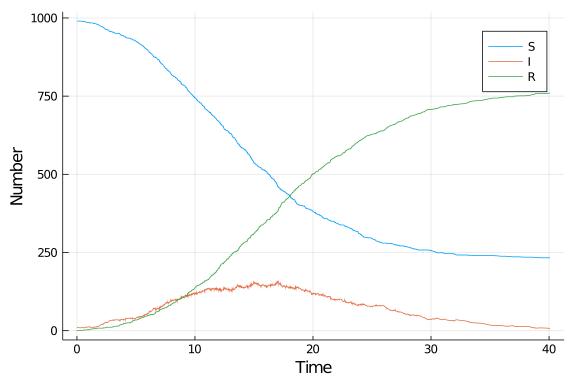
\includegraphics[width=\linewidth]{C:/Users/sdwfr/Projects/sir/sir-julia/pdf/jump_process_gillespie/jl_wmrR7I/jump_gillespie_11_1.pdf}

\subsection{Benchmarking}

\begin{lstlisting}
(*@\HLJLnd{@benchmark}@*) (*@\HLJLnf{ssa}@*)(*@\HLJLp{(}@*)(*@\HLJLn{u0}@*)(*@\HLJLp{,}@*)(*@\HLJLn{sir{\_}rates}@*)(*@\HLJLp{,}@*)(*@\HLJLn{sir{\_}transitions}@*)(*@\HLJLp{,}@*)(*@\HLJLn{p}@*)(*@\HLJLp{,}@*)(*@\HLJLn{tmax}@*)(*@\HLJLp{)}@*)
\end{lstlisting}

\begin{lstlisting}
BenchmarkTools.Trial: 
  memory estimate:  4.88 KiB
  allocs estimate:  40
  --------------
  minimum time:     3.200 (*@\ensuremath{\mu}@*)s (0.00(*@{{\%}}@*) GC)
  median time:      183.050 (*@\ensuremath{\mu}@*)s (0.00(*@{{\%}}@*) GC)
  mean time:        221.174 (*@\ensuremath{\mu}@*)s (13.58(*@{{\%}}@*) GC)
  maximum time:     12.971 ms (98.09(*@{{\%}}@*) GC)
  --------------
  samples:          10000
  evals/sample:     1
\end{lstlisting}



\subsection{Appendix}

\subsubsection{Computer Information}

\begin{verbatim}
Julia Version 1.4.0
Commit b8e9a9ecc6 (2020-03-21 16:36 UTC)
Platform Info:
  OS: Windows (x86_64-w64-mingw32)
  CPU: Intel(R) Core(TM) i7-8550U CPU @ 1.80GHz
  WORD_SIZE: 64
  LIBM: libopenlibm
  LLVM: libLLVM-8.0.1 (ORCJIT, skylake)
Environment:
  JULIA_NUM_THREADS = 4

\end{verbatim}

\subsubsection{Package Information}

\begin{verbatim}
Status `~\.julia\environments\v1.4\Project.toml`
[46ada45e-f475-11e8-01d0-f70cc89e6671] Agents 3.0.0
[b19378d9-d87a-599a-927f-45f220a2c452] ArrayFire 1.0.6
[c52e3926-4ff0-5f6e-af25-54175e0327b1] Atom 0.12.10
[6e4b80f9-dd63-53aa-95a3-0cdb28fa8baf] BenchmarkTools 0.5.0
[be33ccc6-a3ff-5ff2-a52e-74243cff1e17] CUDAnative 3.0.4
[3a865a2d-5b23-5a0f-bc46-62713ec82fae] CuArrays 2.0.1
[717857b8-e6f2-59f4-9121-6e50c889abd2] DSP 0.6.6
[2445eb08-9709-466a-b3fc-47e12bd697a2] DataDrivenDiffEq 0.2.0
[a93c6f00-e57d-5684-b7b6-d8193f3e46c0] DataFrames 0.20.2
[aae7a2af-3d4f-5e19-a356-7da93b79d9d0] DiffEqFlux 1.8.1
[41bf760c-e81c-5289-8e54-58b1f1f8abe2] DiffEqSensitivity 6.13.0
[6d1b261a-3be8-11e9-3f2f-0b112a9a8436] DiffEqTutorials 0.1.0
[0c46a032-eb83-5123-abaf-570d42b7fbaa] DifferentialEquations 6.13.0
[31c24e10-a181-5473-b8eb-7969acd0382f] Distributions 0.23.2
[634d3b9d-ee7a-5ddf-bec9-22491ea816e1] DrWatson 1.10.2
[587475ba-b771-5e3f-ad9e-33799f191a9c] Flux 0.10.4
[0c68f7d7-f131-5f86-a1c3-88cf8149b2d7] GPUArrays 3.1.0
[28b8d3ca-fb5f-59d9-8090-bfdbd6d07a71] GR 0.48.0
[523d8e89-b243-5607-941c-87d699ea6713] Gillespie 0.1.0
[7073ff75-c697-5162-941a-fcdaad2a7d2a] IJulia 1.21.2
[e5e0dc1b-0480-54bc-9374-aad01c23163d] Juno 0.8.1
[961ee093-0014-501f-94e3-6117800e7a78] ModelingToolkit 3.0.2
[429524aa-4258-5aef-a3af-852621145aeb] Optim 0.20.6
[1dea7af3-3e70-54e6-95c3-0bf5283fa5ed] OrdinaryDiffEq 5.34.1
[91a5bcdd-55d7-5caf-9e0b-520d859cae80] Plots 1.0.12
[e6cf234a-135c-5ec9-84dd-332b85af5143] RandomNumbers 1.4.0
[c5292f4c-5179-55e1-98c5-05642aab7184] ResumableFunctions 0.5.1
[428bdadb-6287-5aa5-874b-9969638295fd] SimJulia 0.8.0
[05bca326-078c-5bf0-a5bf-ce7c7982d7fd] SimpleDiffEq 1.1.0
[f3b207a7-027a-5e70-b257-86293d7955fd] StatsPlots 0.14.5
[789caeaf-c7a9-5a7d-9973-96adeb23e2a0] StochasticDiffEq 6.19.2
[44d3d7a6-8a23-5bf8-98c5-b353f8df5ec9] Weave 0.9.4
[37e2e46d-f89d-539d-b4ee-838fcccc9c8e] LinearAlgebra
[cf7118a7-6976-5b1a-9a39-7adc72f591a4] UUIDs
\end{verbatim}



\end{document}
